\documentclass[landscape,a2,final,10pt]{issposter}

% If you encounter errors like "No room for a new ...", use etex (needs
% to be the first package. This happens, if too many registers are used
% because of too many packages or too many complex packages (like e.g. 
% tikz, pstricks and longtable). etex extends the number of registers.
% etex has to be the first package to be loaded!
% \usepackage{etex}

\usepackage[latin1]{inputenc}
\usepackage{multicol}
\usepackage{graphicx,wrapfig,lipsum}
\usepackage[ngerman]{babel}
\usepackage{amsmath}
\usepackage{amsfonts}
\usepackage{amssymb}
\usepackage{dsfont}
\usepackage[justification=centering]{caption}

% If you want to use latex, dvips and ps2pdf, use hyperref to get correct
% page sizes. With hyperref, you won't have to specify them on the command
% line.
% \usepackage[pdfpagemode=UseNone,dvips,pdfborder={0 0 0}]{hyperref}

% \usepackage{tikz} % nice graphics, also used for the fancy boxes

% \usepackage{pstricks,pst-plot,pst-node} % nice graphics with PS
% \psset{unit=3mm,nodesep=1.5,linewidth=.3}
% Use auto-pst-pdf, to use PSTricks with pdflatex. In this case,
% you have to add --shell-escape to your pdflatex command line.
% \usepackage{auto-pst-pdf}

% Set the font sizes. Change these, if you want to change only one or two.
% Use the font size options of the document class (14pt, 17pt, 20pt, 15pt, 30pt, 36pt),
% if you want to change all the sizes at once.
\renewcommand{\titlesize}{\LARGE}
\renewcommand{\sectionsize} {\Large}
\renewcommand{\authorsize}{\Large}
\renewcommand{\instsize}{\large}
\renewcommand{\figurename}{Fig.}
\usepackage[font=scriptsize,labelfont=bf]{caption}
\setlength{\abovecaptionskip}{5pt plus 3pt minus 2pt} % Chosen fairly arbitrarily



% Insert your data
\title{\MakeUppercase{Great Barrier Reef: Invasive Starfish Detector}}
\author{Nick Wagner and David Unger}
\institute{Institute of Signal Processing and System Theory, University of Stuttgart, Germany}
\conference{\normalsize \textbf{Deep Learning Lab 2022}, February 8, Stuttgart, Germany }

% -----------------------------------------------------------------------------
\begin{document}
\maketitle

% Justified text sometimes looks strange in narrow columns
\raggedright

\begin{multicols}{3}
%%%%%%%%%%%%%%%%%%%%%%%%%%%%%%%%%%%%%%%%%%%%%%%%
\section{Problem Statement}
    \textbf{Abstract}\\
    \begin{small} The Great Barrier Reef in Australia is known world-wide for its diverse animal and coral species.
        Recently, the overpopulation of the coral-eating crown-of-thorns starfish threatens the existance of many corals.
        To allow divers to efficiently remove these star fishes from the corals, we develop an object detection algorithm. \newline
        The algorithm is based on the ''YOLO''--framework and takes video sequences as input, detects the starfishes and draws bounding boxes around them.
    \bigskip   
    \end{small}
    % starfish image 
    \begin{wrapfigure}{r}{0pt}
    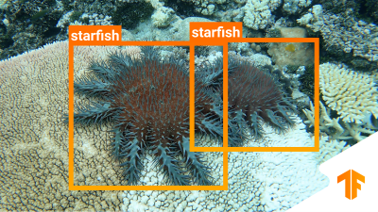
\includegraphics[scale=0.8]{1_starfishes.png}
    \caption{test123}
    \end{wrapfigure} 

    \textbf{Dataset}
    \begin{small}
    \begin{itemize}
        \item \raisebox{-0.6ex}{\~{}}23000 images\\ from 3 video sequences
        \item bounding box labels from csv\\
        \item binary problem
    \end{itemize}
    \end{small}
    \hfill \break
    \hfill \break
    \columnbreak
%%%%%%%%%%%%%%%%%%%%%%%%%%%%%%%%%%%%%%%%%%%%%%%%
    \section{Architecture}
        \begin{itemize}
            \item Text item
            \item Text item
            \item Text item
        \end{itemize}
    \columnbreak
%%%%%%%%%%%%%%%%%%%%%%%%%%%%%%%%%%%%%%%%%%%%%%%%    
    \section{Network Output}
        \begin{itemize}
            \item Text item
            \item Text item
            \item Text item
        \end{itemize}
    \columnbreak
\end{multicols}


\rule{\textwidth}{8pt}

\begin{multicols}{3}
%%%%%%%%%%%%%%%%%%%%%%%%%%%%%%%%%%%%%%%%%%%%%%%%
\section{Input Pipeline}
        \begin{small}Compared to a classification network, a detection network requires a more complicated input pipeline. This mainly comes from the 
        labels which are dependent on the image content and that change, if the image is scaled, rotated, cropped or flipped.Therefore, the input pipeline consists of the following steps:
        \begin{itemize}
            \item CSV loading
            \item Bounding box text to grid conversion
            \item Image reading
            \item Image resizing
            \item Image augmentation
            \item Image visualization
        \end{itemize}
        \end{small}
       
    \columnbreak
%%%%%%%%%%%%%%%%%%%%%%%%%%%%%%%%%%%%%%%%%%%%%%%%
    \section{Loss Function}
        \begin{small} To ensure that the network learns the bounding boxes as represented by the ground truth labels, 
        using a standard loss function is not sufficient. Therefore, the loss function from the YOLO paper is used and adapted 
        that it fits the described problem setup.
        
        
        The four parts of our loss function are the following and summed up during training 
        \begin{itemize}
            \item Objectness loss: \quad $l_{obj} = \lambda_{obj} \sum_{i=0}^{(S-1)^2} \mathds{1}_{i}^{obj} (1 - \hat{p}_i)^2  $
            \item No object loss: \quad \quad $l_{noobj} = \lambda_{noobj} \sum_{i=0}^{(S-1)^2} \mathds{1}_{i}^{noobj} (0 - \hat{p}_i)^2  $
            \item BBox center loss: \quad $l_{center} = \lambda_{center} \sum_{i=0}^{(S-1)^2} \mathds{1}_{i}^{obj} [(x_i - \hat{x}_i)^2 + (y_i - \hat{y}_i)^2] $
            \item BBox size loss: \quad \quad$l_{size} = \lambda_{size} \sum_{i=0}^{(S-1)^2} \mathds{1}_{i}^{obj} [(\sqrt{w_i} - \sqrt{\hat{w}_i})^2 + (\sqrt{h_i} - \sqrt{\hat{h}_i})^2] $
        \end{itemize}

        The loss term weightings $\lambda$ are determined in a way, that all loss terms are in a 
        similar range and therefore are optimized in a similar strength.

        \end{small}
    \columnbreak
%%%%%%%%%%%%%%%%%%%%%%%%%%%%%%%%%%%%%%%%%%%%%%%%    
    \section{Challenge}
        \begin{itemize}
            \item Text item
            \item Text item
            \item Text item
        \end{itemize}
    \columnbreak
\end{multicols}
\end{document}


